\documentclass[../paper.tex]{subfiles}
\begin{document}
\section{Эксперименты}
%
Вычисление значений функции $g_{m,n}(z)$ аналитическим способом, рассмотренным в разделе \ref{analytic-g}, требует использования длинной арифметики
и вычисления большого количества членов ряда. Это приводит к очень низкой скорости построения оценки. 

Для построения оценок численными методами мы использовали следующие параметры
\begin{enumerate}
	\item Равномерная сетка по $x$, состоящая из 1000 точек, минимальная точка: $0{,}05$, максимальная точка: $100$.
	\item Равномерная сетка по $z$, состоящая из 10~000 точек, минимальная точка: $0{,}05$, максимальная точка: $1000$.
	\item Параметр $m$ от $-5$ до $5$ включительно.
	\item Параметр $n$ от $-5$ до $5$ включительно.
	\item Параметр регуляризации $\alpha$: $0{,}1$.
\end{enumerate}.

Опишем графики, приведенные ниже:
\begin{enumerate}
	\item На графике \ref{comp-loss} показано сравнение различных функций ошибок для метода градиентного спуска.
		А именно, приведены графики $\int_0^\infty K(x,z)g_{0,-3}(z)dz$, где $g_{0,-3}$ получено с использованием различных функций ошибок.
		Также приведен график $\psi_{0,-3}$.
	\item На графике \ref{comp-method} изображено сравнение различных методов решения уравнения и приведена целевая функция.
	\item На графиках \ref{norm}, \ref{chisq} изображена оценка для некоторых распределений $X$, полученная методом МНК--оптимизации с $l_2$--регуляризацией.
	\item На графиках \ref{est-lse}, \ref{est-it}, \ref{est-l2} изображены оценки, 
		полученные разными методами, для смеси двух нормальных распределений: $\mathcal{N}(1, 1/4)$ и $\mathcal{N}(3, 1/2)$.
		На этих графиках реконструкцией называется аппроксимация плотности, приведенная в уравнении (\ref{eq:reconstruction}), оценкой --- оценка, указанная в формуле (\ref{eq:estimation}). Также используется поправка, рассмотренная в разделе \ref{correction}.
\end{enumerate}

\begin{figure}[h]
	\begin{minipage}{0.48\textwidth}
		\centering
		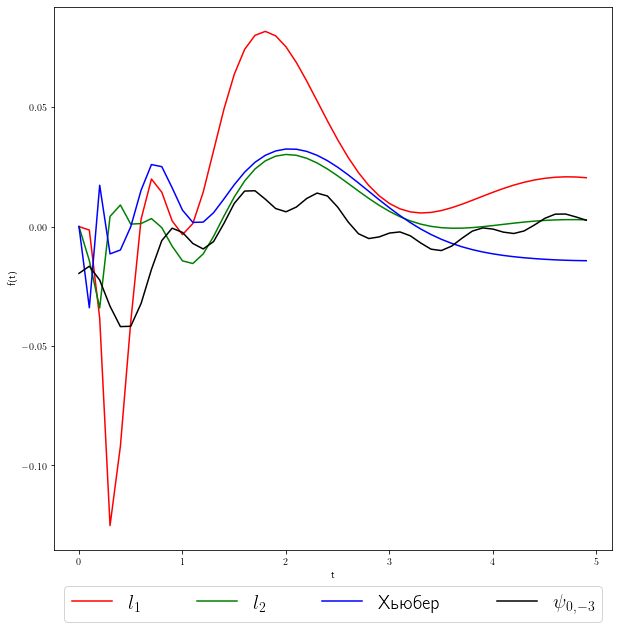
\includegraphics[width=\textwidth]{comp-loss}
		\caption{Сравнение подгонки вейвлета $\psi_{0,-3}(x)$ функциями $g_{0,-3}(z)$, полученными методом градиентного спуска с различными функциями потерь}
		\label{comp-loss}
	\end{minipage}\hfill
	\begin{minipage}{0.48\textwidth}
		\centering
		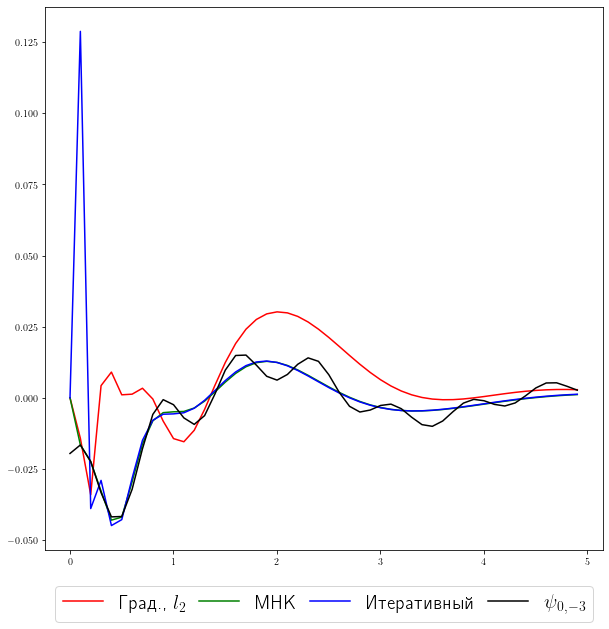
\includegraphics[width=\textwidth]{comp-method}
		\caption{Сравнение подгонки вейвлета $\psi_{0,-3}(x)$ функциями $g_{0,-3}$, полученными итеративным методом, градиентным спуском и МНК-оценкой}
		\label{comp-method}
	\end{minipage}\hfill
\end{figure}

\begin{figure}[h]
	\begin{minipage}{0.48\textwidth}
		\centering
		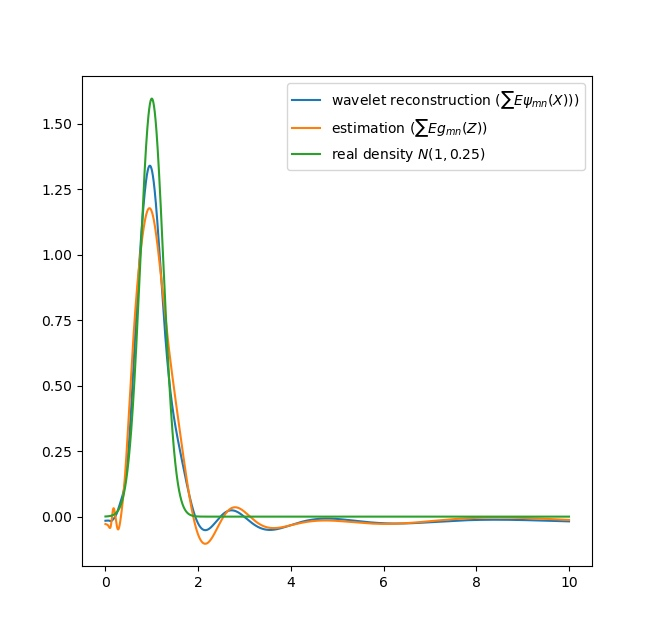
\includegraphics[width=\textwidth]{norm}
		\caption{$X \sim \mathcal{N}(0, 1)$}
		\label{norm}
	\end{minipage}\hfill
	\begin{minipage}{0.48\textwidth}
		\centering
		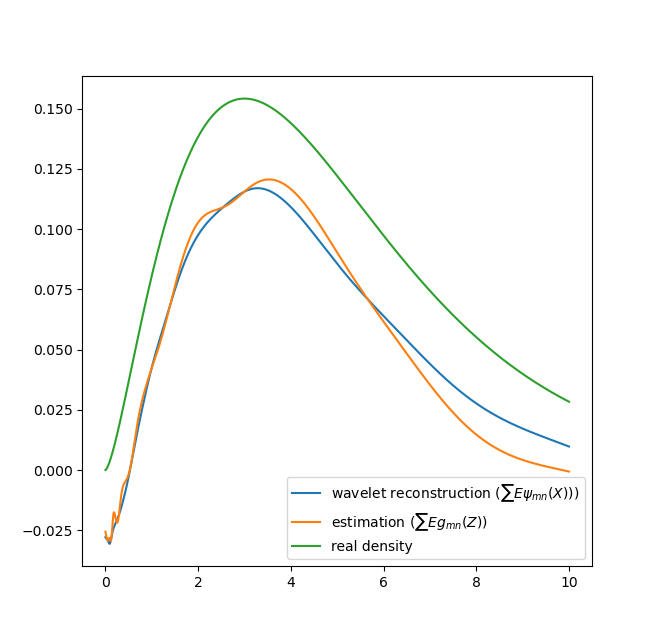
\includegraphics[width=\textwidth]{chisq}
		\caption{$X \sim \chi^2_5$}
		\label{chisq}
	\end{minipage}\hfill
\end{figure}

\begin{figure}[h]
	\begin{minipage}{0.48\textwidth}
		\centering
		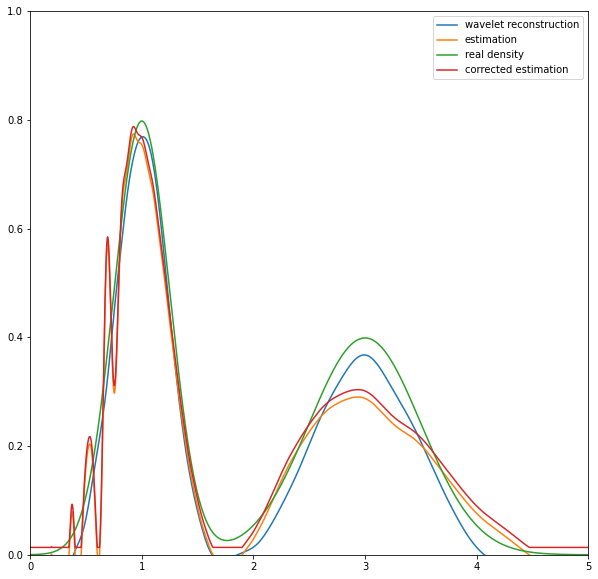
\includegraphics[width=\textwidth]{est-lse}
		\caption{МНК-оценка для смеси нормальных распределений}
		\label{est-lse}
	\end{minipage}\hfill
	\begin{minipage}{0.48\textwidth}
		\centering
		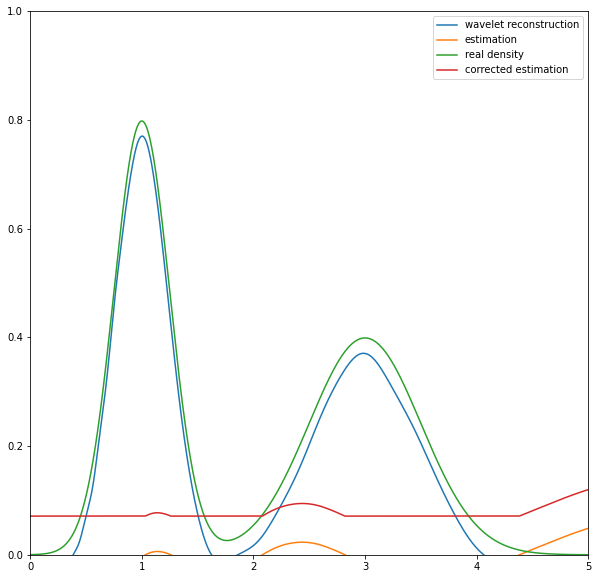
\includegraphics[width=\textwidth]{est-it}
		\caption{Оценка итеративным методом для смеси нормальных распределений}
		\label{est-it}
	\end{minipage}\hfill
\end{figure}

\begin{figure}[h]
	\begin{minipage}{0.48\textwidth}
		\centering
		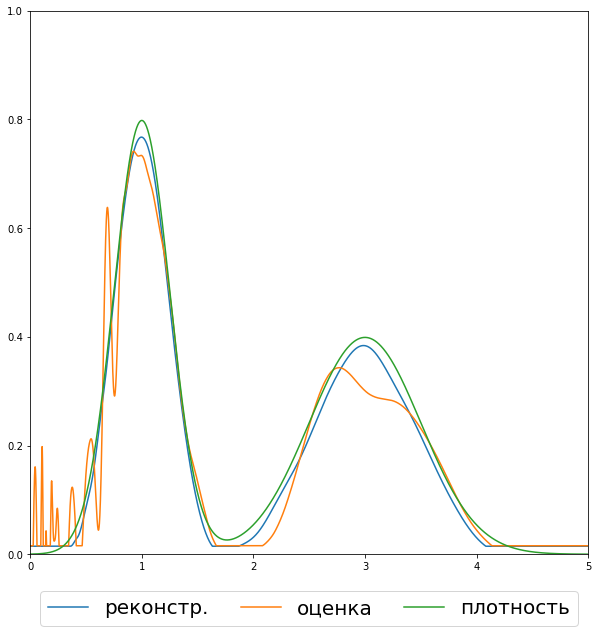
\includegraphics[width=\textwidth]{est-l2}
		\caption{Оценка методом градиентного спуска для смеси нормальных распределений}
		\label{est-l2}
	\end{minipage}\hfill
\end{figure}
\end{document}
